\documentclass[a0paper,portrait]{tikzposter}

\usepackage{booktabs}
\usepackage{mathtools}
\usepackage{tikz-cd}
\usepackage[export]{adjustbox}
\usepackage{amsfonts}
\usepackage[capitalise]{cleveref}
\usepackage{subcaption}
\usepackage{wrapfig}

\tikzposterlatexaffectionproofoff
\usetheme{Rays}
\usenotestyle{VerticalShading}

\usetikzlibrary{arrows}
\usetikzlibrary{arrows.meta}

\AtBeginEnvironment{tikzfigure}{\captionsetup{type=figure}}

\makeatletter
\def\title#1{\gdef\@title{\scalebox{\TP@titletextscale}{%
      \begin{minipage}[t]{\linewidth}
        \centering
        #1
        \par
        \vspace{0.5em}
      \end{minipage}%
    }}}
\makeatother

\makeatletter
\newcounter{tablecounter}
\newenvironment{tikztable}[1][]{
  \def \rememberparameter{#1}
  \vspace{10pt}
  \refstepcounter{tablecounter}
  \begin{center}
  }{
    \ifx\rememberparameter\@empty
    \else
    \\[10pt]
    {\small Tab.~\thetablecounter: \rememberparameter}
    \fi
  \end{center}
}
\makeatother

\title{Weighted Model Counting with Conditional Weights for Bayesian Networks}
\author{Paulius Dilkas, Vaishak Belle}
\institute{University of Edinburgh, Edinburgh, UK\\
  \texttt{p.dilkas@sms.ed.ac.uk}, \texttt{vaishak@ed.ac.uk}}

\begin{document}
\maketitle

\begin{columns}

  \column{0.5}

  \block{Abstract}{
    \textbf{Weighted model counting (WMC)} has emerged as the \textbf{unifying
      inference mechanism} across many (probabilistic) domains. Encoding an
    inference problem as an instance of WMC typically \textbf{necessitates
      adding extra literals and clauses}. This is partly so because the
    predominant definition of WMC assigns weights to models based on weights on
    literals, and this severely restricts what probability distributions can be
    represented. We develop a \textbf{measure-theoretic perspective} on WMC and
    propose a way to encode conditional weights on literals analogously to
    conditional probabilities. This representation can be as succinct as
    standard WMC with weights on literals but can also expand as needed to
    represent probability distributions with less structure. To demonstrate the
    performance benefits of conditional weights over the addition of extra
    literals, we develop a \textbf{new WMC encoding for Bayesian networks}
    \texttt{cw} and adapt a state-of-the-art WMC algorithm \textsf{ADDMC} to the
    new format. Our experiments show that the new encoding significantly
    improves the performance of the algorithm on most benchmark instances.
  }

  \block{WMC as a Measure on a Boolean Algebra}{
    Traditionally, WMC is seen as a \textbf{generalisation of propositional
      model counting}. Here we provide a measure-theoretic definition, the main
    benefit of which is that it allows us to \textbf{define weights more
      flexibly} and results in \textbf{significantly smaller encodings}. While
    measures on Boolean algebras have been studied before, other definitions are
    new. For any set $U$, $2^{2^U}$ (i.e., the powerset of the powerset of $U$)
    is the Boolean algebra that directly corresponds to \textbf{all possible
      propositional formulas} constructable from $a$ and $b$. A \textbf{measure}
    on $2^{2^U}$ is a function $\mu\colon 2^{2^U} \to \mathbb{R}_{\ge 0}$ such
    that
    \coloredbox{
      \begin{itemize}
      \item $\mu(\bot) = 0$, and
      \item $\mu(a \lor b) = \mu(a) + \mu(b)$ for all $a, b \in 2^{2^U}$
        whenever $a \land b = \bot$.
      \end{itemize}
    }
    A \textbf{weight function} is a function $\nu\colon 2^U \to \mathbb{R}_{\ge
      0}$. A weight function is \textbf{factored} if $\nu = \prod_{x \in U}
    \nu_x$ for some functions $\nu_x\colon 2^{\{x\}} \to \mathbb{R}_{\ge 0}$, $x
    \in U$. We say that a weight function $\nu\colon 2^U \to \mathbb{R}_{\ge 0}$
    \textbf{induces} a measure $\mu_\nu\colon 2^{2^U} \to \mathbb{R}_{\ge 0}$ if
    \[
      \mu_\nu(x) = \sum_{\{u\} \le x} \nu(u).
    \]
    Finally, a measure $\mu\colon 2^{2^U} \to \mathbb{R}_{\ge 0}$ is
    \textbf{factorable} if there exists a factored weight function $\nu\colon 2^U
    \to \mathbb{R}_{\ge 0}$ that induces $\mu$. In this formulation, WMC
    corresponds to \textbf{the process of calculating the value of $\mu_\nu(x)$}
    for some $x \in 2^{2^U}$ with a given definition of $\nu$. Moreover,
    \textbf{classical WMC is only able to evaluate factorable measures}.

    \innerblock{Relation to the Classical (Logic-Based) View of WMC}{
      The classical definition of WMC relies on a \textbf{weight function over
        the literals} of a propositional theory. Let $\mathcal{L}$ be a
      propositional logic with two atoms $a$ and $b$ and $w\colon \{ a, b, \neg
      a, \neg b \} \to \mathbb{R}_{\ge 0}$ a weight function defined as $w(a) =
      0.3$, $w(\neg a) = 0.7$, $w(b) = 0.2$, $w(\neg b) = 0.8$. Furthermore, let
      $\Delta$ be a theory in $\mathcal{L}$ with a sole axiom $a$. Then $\Delta$
      has two models: $\{ a, b \}$ and $\{ a, \neg b \}$ and its WMC is
      \begin{equation} \label{eq:wmc_example}
        \mathrm{WMC}(\Delta) = \sum_{\omega \models \Delta} \prod_{\omega \models l} w(l) = w(a)w(b) + w(a)w(\neg b) = 0.3,
      \end{equation}
      i.e., we \textbf{sum over all models} entailed by the theory, and the
      weight of each model is \textbf{the product of the weights of all literals
        in it}. Alternatively, we can define $\nu_a\colon 2^{\{a\}} \to
      \mathbb{R}_{\ge 0}$ as $\nu_a(\{ a \}) = 0.3$, $\nu_a(\emptyset) = 0.7$
      and $\nu_b\colon 2^{\{b\}} \to \mathbb{R}_{\ge 0}$ as $\nu_b(\{ b \}) =
      0.2$, $\nu_b(\emptyset) = 0.8$. Let $\mu$ be the measure on $2^{2^U}$
      induced by $\nu = \nu_a \cdot \nu_b$. Then, equivalently to
      \cref{eq:wmc_example}, we can write
      \begin{align*}
        \mu(a) &= \nu(\{ a, b \}) + \nu(\{ a \}) \\
               &= \nu_a(\{a\})\nu_b(\{b\}) + \nu_a(\{a\})\nu_b(\emptyset) = 0.3.
      \end{align*}
      Thus, one can equivalently think of WMC as summing over \textbf{models of
        a theory} or over \textbf{atoms below an element} of a Boolean algebra.
    }
  }

  \begin{subcolumns}
    \subcolumn{0.44}
    \block{}{
      \begin{center}
        
\includegraphics[height=200pt]{logo_inf.png}
        
\includegraphics[height=200pt]{logo_ecr.png}
        
\includegraphics[height=100pt]{logo_ukri.png}
      \end{center}
    }
    \subcolumn{0.56}
    \note[width=0.29\linewidth,targetoffsetx=0.152\linewidth,targetoffsety=0.01\textheight]{
      For instance, the Boolean algebra $2^{2^{\{a, b\}}}$ can be visualised as
      \[
        \begin{tikzcd}[ampersand replacement=\&, column sep=tiny]
          \& \& \& \& \& \top \ar[dlll,dash,gray] \ar[dl,dash,gray]
          \ar[dr,dash,gray] \ar[drrr,dash,gray] \& \& \& \\
          \& \& a \lor b \& \& b \to a \& \& a \to b \& \& \neg a \lor \neg
          b \\
          a \ar[urr,dash,gray] \ar[urrrr,dash,gray] \& \& b \ar[u,dash,gray]
          \ar[urrrr,dash,gray] \& \& a \leftrightarrow b \ar[u,dash,gray]
          \ar[urr,dash,gray] \& \& a + b \ar[ullll,dash,gray] \ar[urr,dash,gray]
          \& \& \neg b \ar[ullll,dash,gray] \ar[u,dash,gray] \& \& \neg a
          \ar[ullll,dash,gray] \ar[ull,dash,gray] \\
          \& \& \fbox{$a \land b$} \ar[ull,dash,gray] \ar[u,dash,gray]
          \ar[urr,dash,gray] \& \& \fbox{$a \land \neg b$} \ar[ullll,dash,gray]
          \ar[urr,dash,gray] \ar[urrrr,dash,gray] \& \& \fbox{$\neg a \land b$}
          \ar[ullll,dash,gray] \ar[u,dash,gray] \ar[urrrr,dash,gray] \& \&
          \fbox{$\neg a \land \neg b$} \ar[ullll,dash,gray] \ar[u,dash,gray]
          \ar[urr,dash,gray] \\
          \& \& \& \& \& \bot. \ar[ulll,dash,gray] \ar[ul,dash,gray]
          \ar[ur,dash,gray] \ar[urrr,dash,gray] \& \& \&
        \end{tikzcd}
      \]
      Boxed elements are the \textbf{atoms} of the algebra.
    }
  \end{subcolumns}

 \column{0.5}

  \block{Example: Encoding Bayesian Networks}{
    \begin{wrapfigure}[8]{r}{0.55\linewidth}
    \begin{tikzfigure}[A Bayesian network with its conditional probability
      tables]
      \begin{subfigure}{0.2\linewidth}
        \centering
        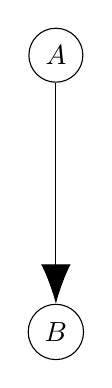
\begin{tikzpicture}[edge from parent/.style={draw,-latex}, level distance=100pt, edge from parent/.style={draw,-{Latex[length=5mm]}}]
          \node[draw,circle] {$A$}
          child {node[draw,circle] {$B$}};
        \end{tikzpicture}
      \end{subfigure}%
      \begin{subfigure}{0.8\linewidth}
        \centering
        \begin{tabular}[t]{cc}
          \toprule
          $a$ & $\Pr(A = a)$ \\
          \midrule
          1 & 0.5 \\
          0 & 0.5 \\
          \bottomrule
        \end{tabular}
        \begin{tabular}[t]{ccc}
          \toprule
          $a$ & $b$ & $\Pr(B = b \mid A = a)$ \\
          \midrule
          1 & 1 & 0.6 \\
          1 & 0 & 0.4 \\
          0 & 1 & 0.1 \\
          0 & 0 & 0.9 \\
          \bottomrule
        \end{tabular}
      \end{subfigure}
    \end{tikzfigure}
    \end{wrapfigure}
    A typical WMC encoding for the pictured Bayesian network needs \textbf{8 variables
    and 17 clauses}. However, the \texttt{cw} weight function only needs \textbf{two
    variables}. Let $U = \{ \lambda_{A=1}, \lambda_{B=1} \}$ be the set of
    variables. Using some simple syntax for manipulating weight functions
    (mostly defined pointwise), we can define the weight function $\nu\colon 2^U
    \to \mathbb{R}_{\ge 0}$ for this network as $\nu \coloneqq \nu_A \cdot
    \nu_B$, where
    \[
      \nu_A = 0.5,
    \]
    and
    \begin{align*}
      \nu_B = 0.6[\lambda_{B=1}] \cdot [\lambda_{A=1}] + 0.4[\neg\lambda_{B=1}] \cdot [\lambda_{A=1}] + 0.1[\lambda_{B=1}] \cdot [\neg\lambda_{A=1}] + 0.9[\neg\lambda_{B=1}] \cdot [\neg\lambda_{A=1}].
    \end{align*}
  }

  \block{Experimental Results}{
    \begin{tikzfigure}[Cumulative numbers of instances solved by combinations of
      algorithms and encodings over time]
      \centering
      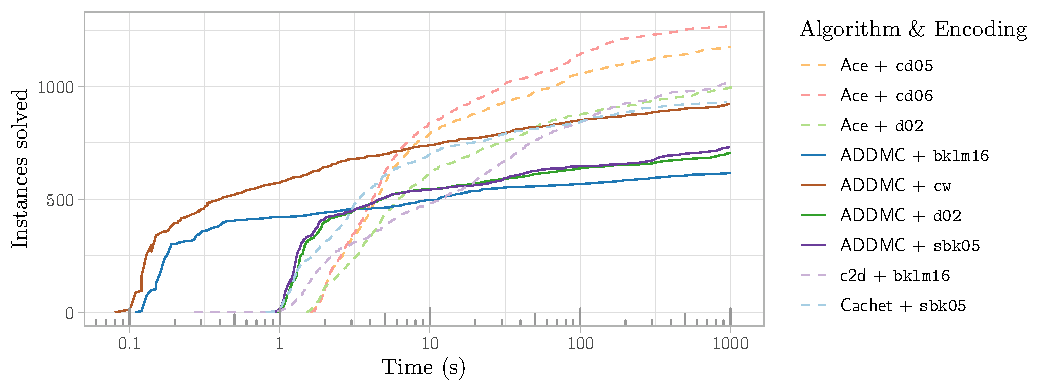
\includegraphics[width=\linewidth]{cumulative}
    \end{tikzfigure}
    \begin{tikzfigure}[An instance-by-instance comparison between
      $\textsf{ADDMC} + \texttt{cw}$ and the best overall combination of
      algorithm and encoding ($\textsf{Ace} + \texttt{cd06}$, on the left) as
      well as the second-best encoding for \textsf{ADDMC} (\texttt{sbk05}, on
      the right)]
      \centering
      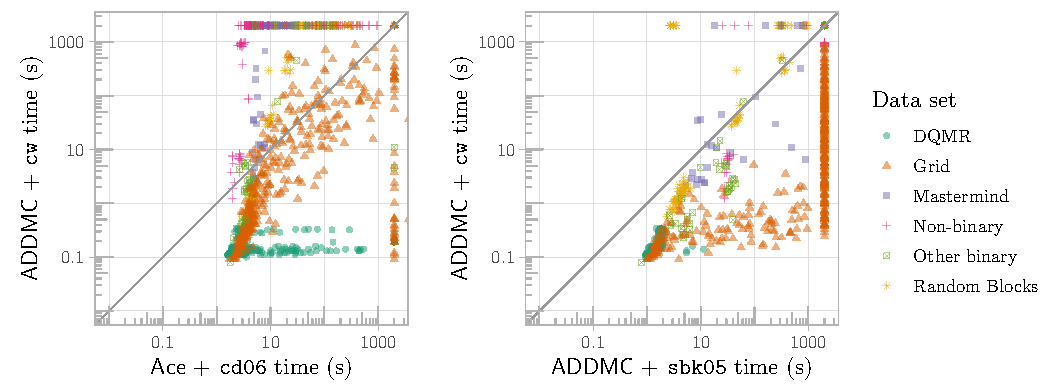
\includegraphics[width=\linewidth]{scatter}
    \end{tikzfigure}
    We compare all six WMC encodings for Bayesian networks when run with both
    \textsf{ADDMC} and the WMC algorithms used in the original papers. The
    cumulative plot shows that \textsf{ADDMC} significantly \textbf{underperforms} when
    combined with any of the \textbf{previous encodings}, but our encoding \texttt{cw}
    significantly \textbf{improves} the performance of \textsf{ADDMC}, making
    $\textsf{ADDMC}+\texttt{cw}$ comparable to many other combinations. The
    scatter plot on the left-hand side adds to this by showing that \texttt{cw}
    is \textbf{particularly promising on certain data sets} such as DQMR and
    Grid networks. The scatter plot on the right-hand side shows that
    \texttt{cw} is better than \texttt{sbk05} (i.e., the second-best encoding
    for \textsf{ADDMC}) on the \textbf{majority of instances}. Seeing how, e.g.,
    DQMR instances are trivial for $\textsf{ADDMC}+\texttt{cw}$ but hard for
    $\textsf{Ace}+\texttt{cd06}$, and vice versa for Mastermind instances, we
    conclude that the best-performing algorithm-encoding combination
    \textbf{depends} significantly \textbf{on} (as-of-yet unknown)
    \textbf{properties of the Bayesian networks}.
  }

  \block{See the Paper for\dots}{
    \begin{itemize}
    \item Theoretical results that establish both the limits and the
      capabilities of classical WMC.
    \item Details of the \texttt{cw} encoding for Bayesian networks.
    \item A more detailed comparison of Bayesian network encodings, including a
      parameterized asymptotic analysis of their growth.
    \end{itemize}
  }

\end{columns}
\end{document}